%!TEX root = SysSpec_ClockPendulumAnalyzer.tex
\subsection{Umsetzung des Zählers} %TODO Counter Realisierung beschreiben
Der Tick-Conter zwischen den Pendeldurchgängen basiert auf einem Freilaufendem Hardware-Zähler, welcher auf dem Tiny K20 Mikrocontrollerboard läuft, getrieben von dem vorhandenen, termperaturkorrigieren 8MHz Quarz, mittels Hardware-Einstellung des CPU-Blocks auf 12MHz erhöht. Diese Erhöhung beruht rein auf Hardware-Einstellungen, die Genauigkeit wird entsprechend nicht beeinflusst.
Um die Schwankungen des Zählers auszugleichen wird der Sekundenpuls des GPS-Moduls über zwei unabhängige IO-Pins genutzt. Eine Leitung am FIX-Pin des GPS-Moduls angeschlossen, für den Fall, dass keine GPS-Verbindung besteht und eine Zweite am PPS-Pin des GPS-Moduls, falls GPS-Verbindung besteht.
Beide Leitungen funktionieren über einen Interrupt der höchsten Priorität. Falls am PPS-Pin Interrupts eingehen, wird der FIX-Pin ignoriert. Beim Umschalten zwischen GPS-Empfang und keinem GPS-Empfang kann daher ein Fehler entstehen. Im Normalbetrieb werden die Interrupts an den IO-Pins, eingehend vom GPS-Modul, dazu genutzt die Differenz zwischen dem vorigen Zählerwert und dem aktuellen Zählerwert zu bilden und so die effektive Frequenz zu ermitteln. Bei Störungen wird die Referenzfrequenz nicht korrigiert und mit dem letzten Wert weitergearbeitet. Um eine Störung festzustwellen wird geprüft, ob die ermittelte Referenz-Frequenz im erlaubten Bereich von +/-100ppm zum erwartenten Wert abweicht.\\ 
Die Pendeldurchgänge werden über einen weiteren IO-Pin über einen Interrupt der höchsten Priorität ermittelt. Dabei wird jede zweite Messung verworfen, um das Pendel immer von der gleichen Seite zu messen. Der ermittelte Zählerwert wird mit der ermittelten Frequenz verrechnet und über die UART-RS232 Schnittstelle gesendet.\\
Die Verrechnungskorrektur erfolgt über folgende Formel:
\[
	T_{abs} = \frac{T_{measured} \cdot f_{ref}}{f_{real}}
\]
\subsubsection{Genauigkeit Referenzfrequenz TinyK20}
Die Genauigkeit der Referenzfrequenz ist mittels statistischer Methoden ermittelt worden. Dazu sind zwei Versuchstreihen durchgeführt worden. Jeweils zwanzig Vergleiche mit dem FIX-Pin als Sekundenpuls, somit ohne GPS-Verbiundung und 20 Messungen mit dem PPS-Pin als Sekundenpuls. Temperatur und Luftfeuchtigkeit sind mit einem Sensirion SHTC1- Sensor ermittelt worden.
Die Frequenzwerte sind dem Debug-Systems aus dem Kinetis Design Studio entnommen, jeweils mit ca zehn Sekunden Pause zwischen zwei Werten. Die ermittelten Daten sind in Tabelle \ref{tab:testvalues} aufgelistet.
\begin{table}[H]
	\centering
	\begin{tabular}{|l|l|} \hline
		\textbf{Werte ohne GPS-Empfang}	& \textbf{Werte mit GPS-Empfang} \\ \hline
		11980515						& 11980579 \\ \hline
		11980483						& 11980569 \\ \hline
		11980481						& 11980569 \\ \hline
		11980487						& 11980577 \\ \hline
		11980527						& 11980577 \\ \hline
		11980493						& 11980575 \\ \hline
		11980532						& 11980578 \\ \hline
		11980539						& 11980581 \\ \hline
		11980500						& 11980582 \\ \hline
		11980546						& 11980577 \\ \hline
		11980505						& 11980578 \\ \hline
		11980511						& 11980570 \\ \hline
		11980518						& 11980585 \\ \hline
		11980520						& 11980585 \\ \hline
		11980517						& 11980582 \\ \hline
		11980521						& 11980581 \\ \hline
		11980559						& 11980584 \\ \hline
		11980555						& 11980589 \\ \hline
		11980529						& 11980590 \\ \hline 
		11980521						& 11980589 \\ \hline
	\end{tabular}
	\caption{Testwerte jeweils ohne- und mit GPS-Empfang}
	\label{tab:testvalues}
\end{table}
Es sind im Anschluss folgende Untersuchungen erfolgt:
\begin{itemize}
	\item Streuung der Daten mit Hilfe eines Histogramms und Box-Plots
	\item sowie eine Prüfung auf die Verteilung mittels QQ-Plot.
	\item Umgebungstemperatur: 23.74°.
	\item Luftfeuchtigkeit: 27.16%
\end{itemize}
Der Boxplot in Abbildung \ref{fig:freq_boxplot} zeigt auf, dass die Genauigkeit des Sekundenpulses des GPS-Modules deutlich von der Genauigkeit des PPS-Signals abweicht. Im vorhandenen Versuch liegt die Streuung ohne GPS-Empfang bei 78ppm während die Streuung mit GPS noch 21ppm beträgt. Die Zahlen entsprechen der Summe de folgender Fehler:
\begin{itemize}
	\item Signals des GPS-Modules.
	\item Registrierung des Interrupts.
	\item Ungenauigkeit des Hardware-Zählers.
	\item Auswerten des Zählerstandes und Differenzbildung. 
\end{itemize}
	\begin{figure}[H]
		\centering
		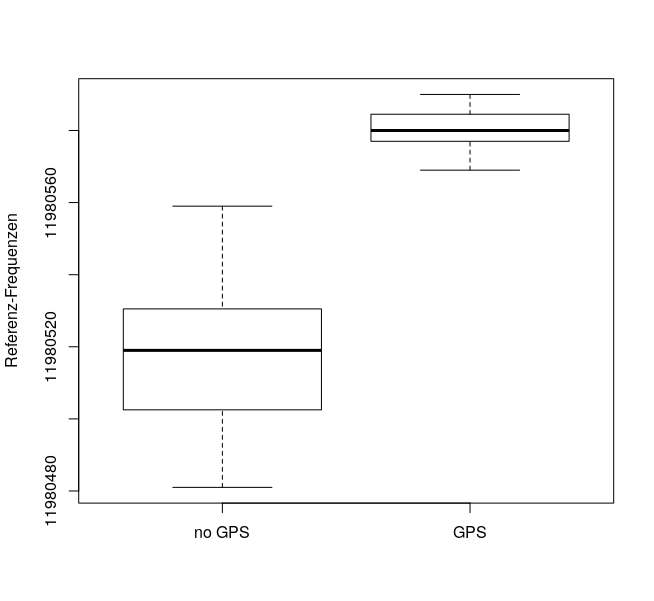
\includegraphics[width=.6\textwidth]{frequencies_boxplot}
		\caption{Boxplot der Versuchsreihen}
		\label{fig:freq_boxplot}
	\end{figure}
%
Weiter kann dem Boxplot entnommen werden, dass die Streuung der Werte gleichmässig um den Median erfolgen und keine Ausreisser vorhanden sind. Dies legt die Vermutung nahe, dass sich die Streuung Normalverteilt verhält, was bedeuten würde, dass sich der Fehler über lange Sicht aufhebt, bis auf eine Konstante Abweichung, welche sich mit der Differenz zwichen Erwartungswert und dem definierten Wert ermitteln lässt. Diese Vermutung ist mit einem Historgramm (Abbildung \ref{fig:freq_histograms}) und einem QQ-Plot (Abbildung \ref{fig:freq_qq_plot}) überprüft worden.
	\begin{figure}[H]
		\centering
		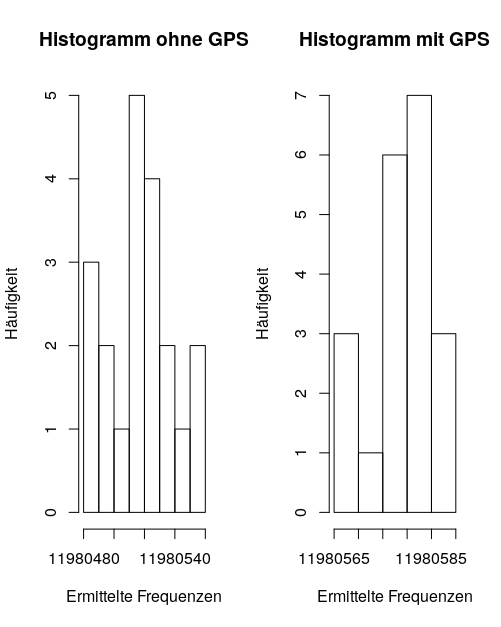
\includegraphics[width=.6\textwidth]{histograms_frequencies}
		\caption{Histogramme der ermittelten Zählerdaten}
		\label{fig:freq_histograms}
	\end{figure}
	Das Histogramm alleine ist bezüglich der Verteilung noch nicht aussagekräftig, dem QQ-Plot kann man anschliessend entnehmen, dass sich die Werte einer Normalverteilung nähern.
	\begin{figure}[H]
		\centering
		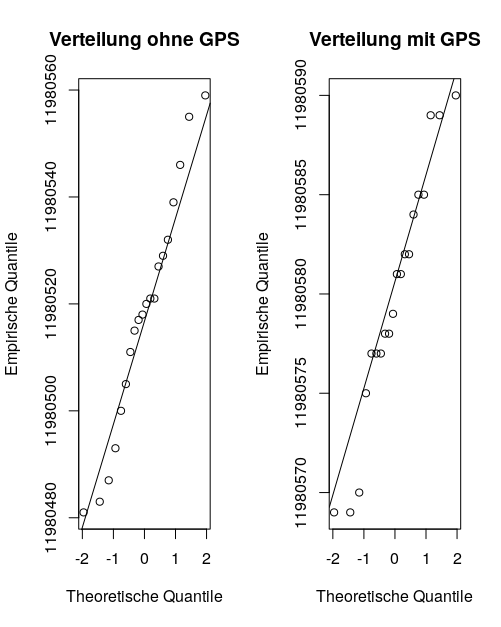
\includegraphics[width=.6\textwidth]{frequencies_qq_plots}
		\caption{QQ-Plots der ermittelten Zählerdaten}
		\label{fig:freq_qq_plot}
	\end{figure}
GPS-Modul und Tiny K20 sind auf einem Board gemeinsam angebracht, ebenfalls auf diesem Board befindet sich die RTC und er Anschluss für den Sensor für die Pendel-Registrierung (Abbildung \ref{fig:hardware_board}).
	\begin{figure}[H]
		\centering
		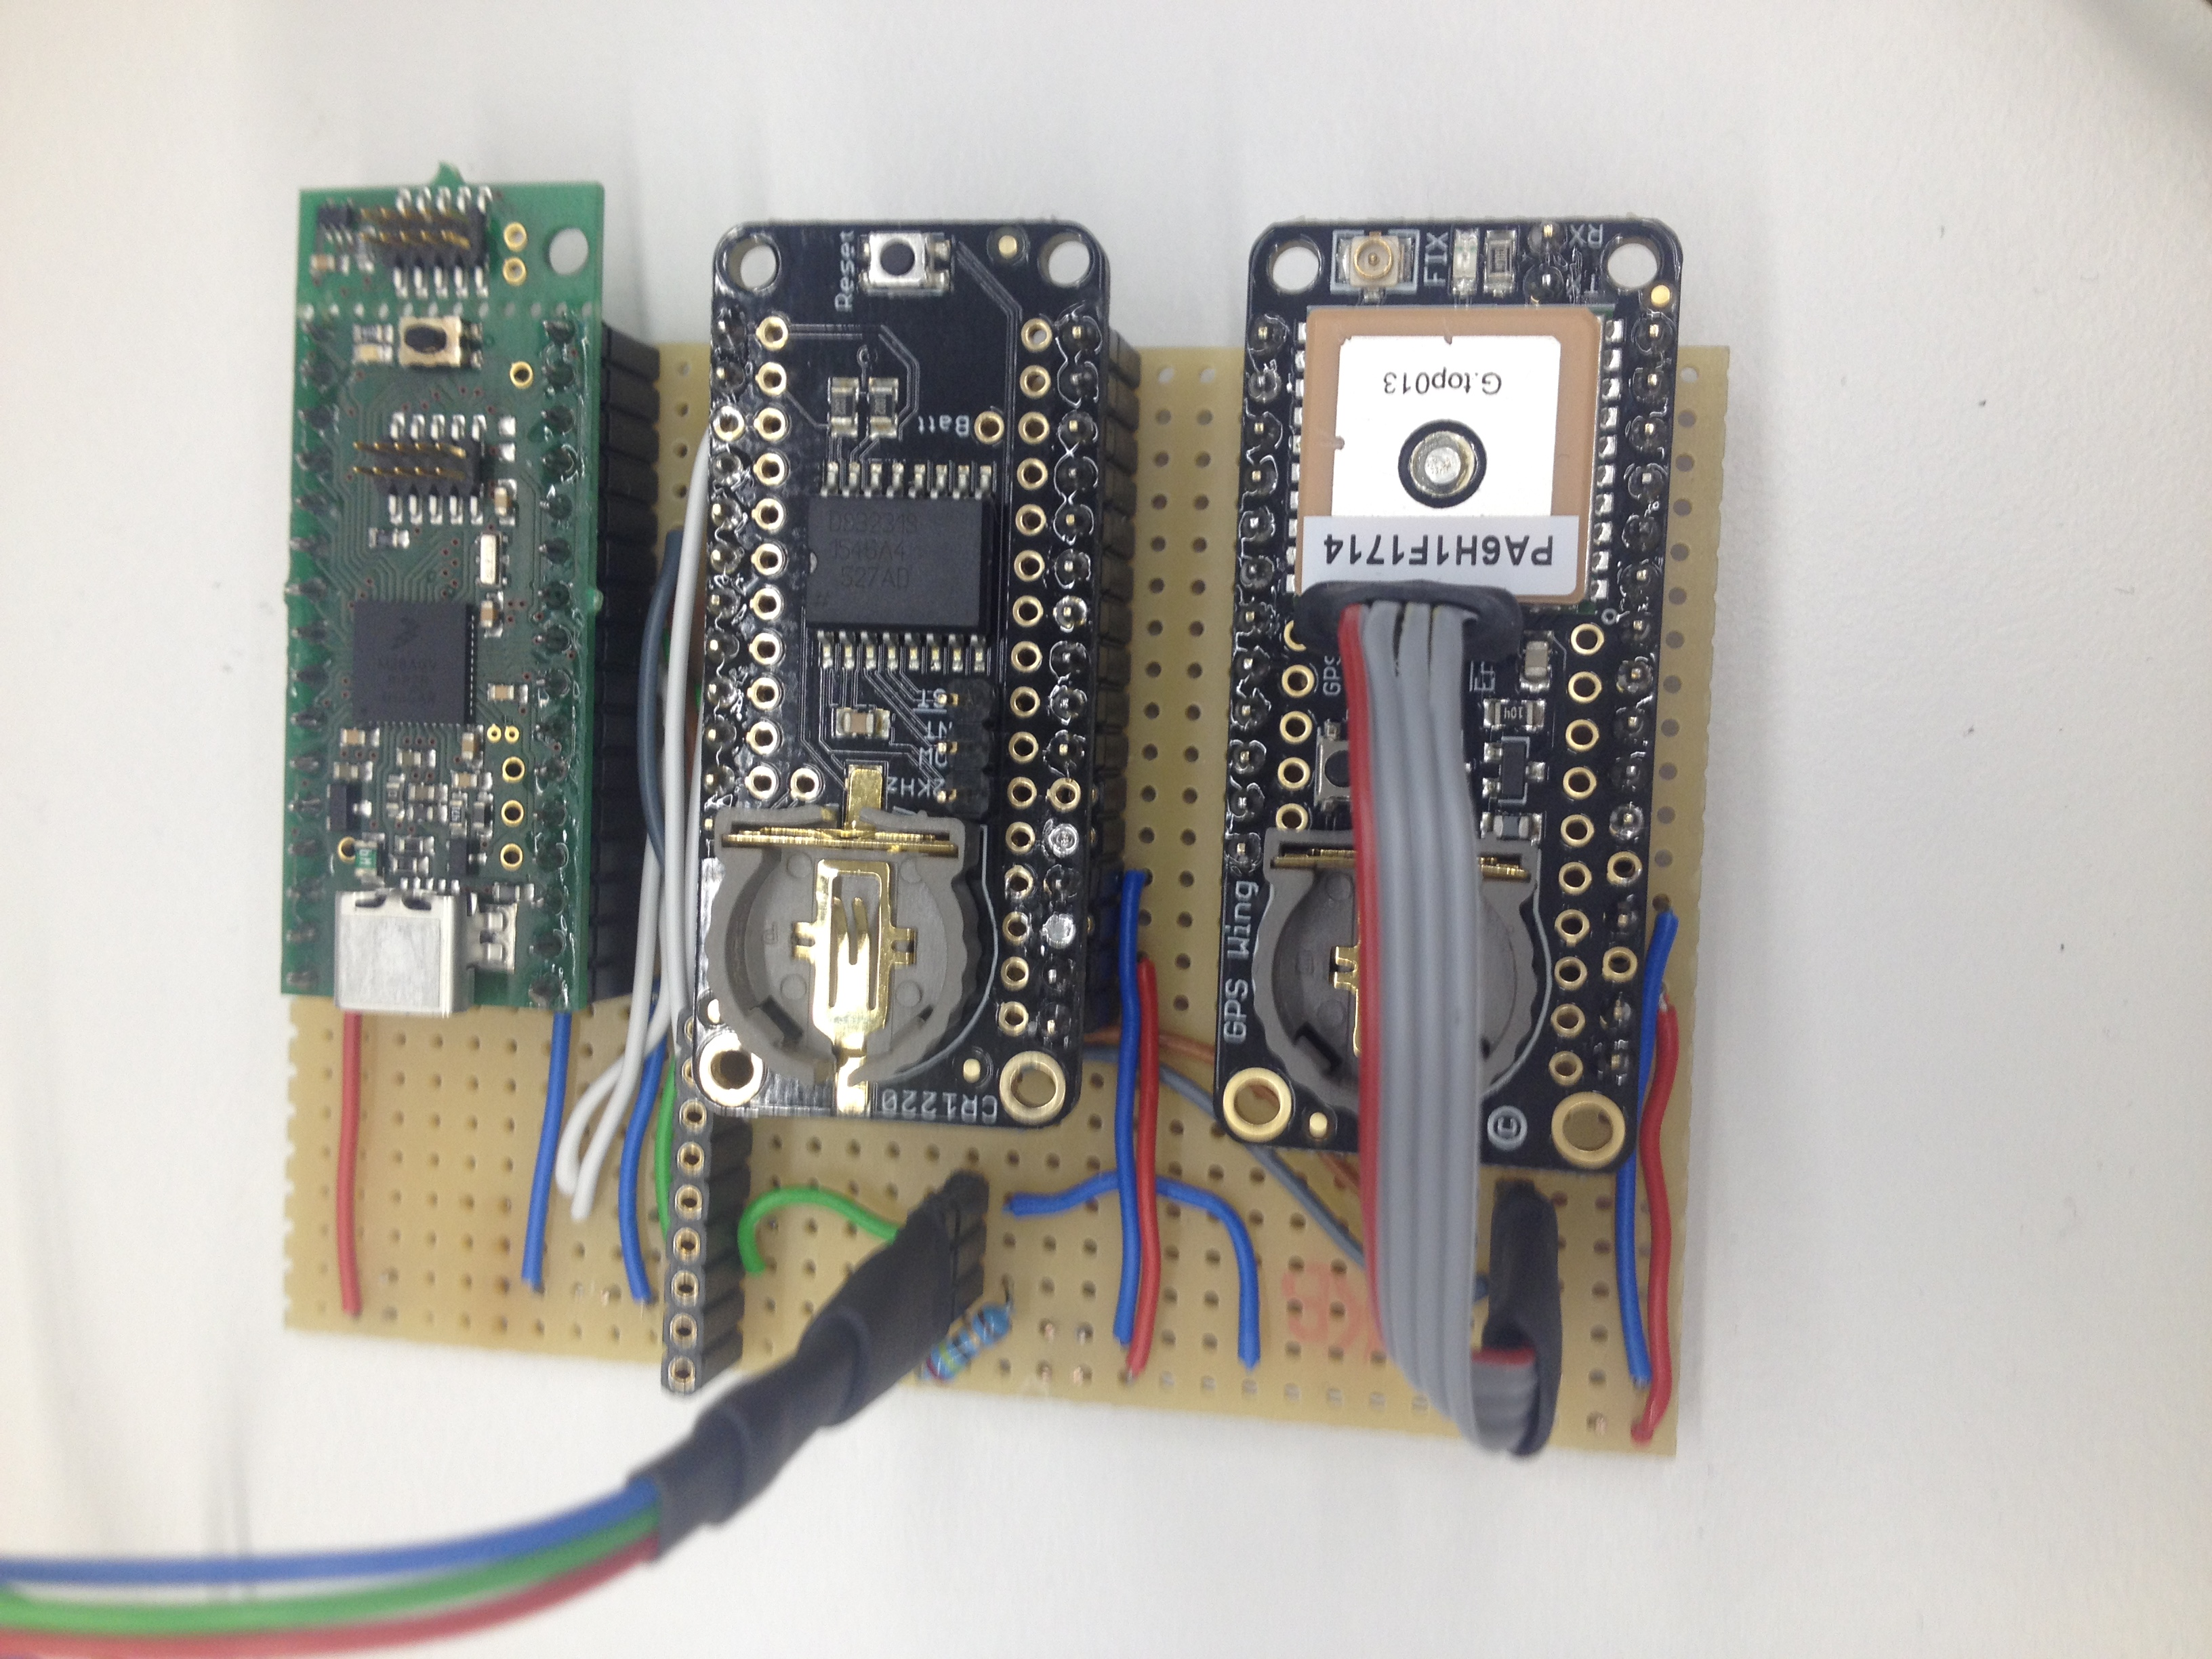
\includegraphics[width=.7\textwidth]{HW_Board_Complete}
		\caption{Gesamtanordnug der Hardware-Komponenten}
		\label{fig:hardware_board}
	\end{figure}